\documentclass[pageno]{jpaper}

\newcommand{\IWreport}{2017}
\newcommand{\quotes}[1]{``#1''}


\widowpenalty=9999

\usepackage[normalem]{ulem}
\usepackage{amsmath}

\begin{document}

\title{Solving the Generalized Form of the Game of Set Efficiently}

\author{Steven Takeshita\\Adviser: Zachary Kincaid}

\date{}
\maketitle

\thispagestyle{empty}
\doublespacing
\begin{abstract}
This paper examines three implementations of a solver to efficiently find sets in the generalized version of the Game of Set. The three techniques are brute force, SMT solver, and dynamic algorithm. The brute force solution is ruled out, as its growth is exponential on small test cases. Through timing tests, it is shown that though a reduction to the SMT solver should create an efficient solution to the NP complete game, the dynamic algorithm approach yields the fastest solver for relatively smaller test cases. Interestingly, the order of growth of the SMT solver follows a linear progression, whereas the dynamic algorithm exponentially grows as parameters are increased, most likely due to its heavy memory usage. At high numbers of values and properties, the SMT solver yields a more efficient solver than the dynamic algorithm. 
\end{abstract}

\section{Introduction}

\subsection{Motivation and Goal}

The Game of Set was created in 1974 and published in 1991. The game consists of $3^4 = 81$ unique cards. Each card has four properties and one of three values. A valid set of three cards is one in which for each property, they all either have the same or different values. See Figure~\ref{fig:SetOverview} for an overview of the game and to see how the properties and values are visually represented for all cards. At the beginning of the game, $12$ cards are shown, and players must locate valid sets. Once a set is found or no set exists, three new cards are added. The person who collected the most sets wins. 

\begin{figure}[htbb]
\centering
\begin{minipage}[b]{.75\linewidth}
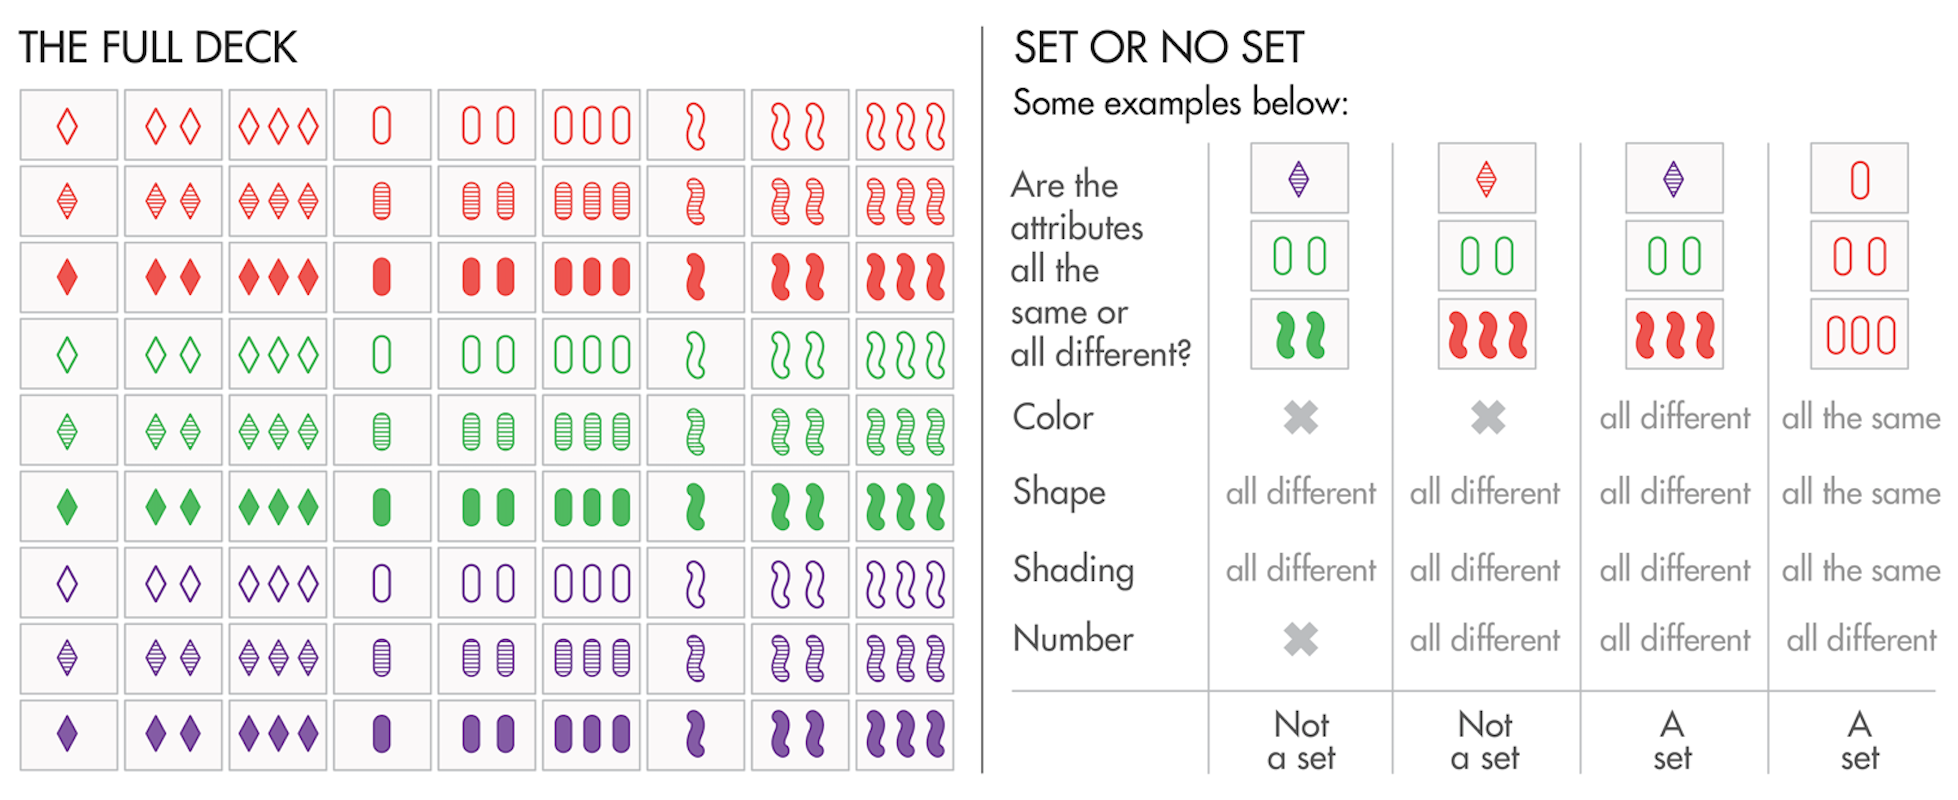
\includegraphics[width=\linewidth]{SetOverview.png}
\caption{Brief Overview of the Game of Set with $v=3$ and $p=4$}
\label{fig:SetOverview}
\end{minipage}
\end{figure}

When I used to play this game with my family, I had difficulty finding sets and always lost to my much faster sister. A natural extension of this game is to determine how fast can a computer find sets, and what are the different ways that we can minimize the time taken. The game itself is relatively limited with only three values and four properties, and therefore generalizing the number of values and properties will make the game much more difficult for a computer to solve. The Game of Set is an interesting problem for dynamic algorithms in that when three new cards are added, the algorithm should be able to build off of previous knowledge. A way to utilize this past information could be helpful in applying similar principles to other problems that could lend itself to dynamic programming. The goal of my project is to create a solver that locates $n$ sets efficiently in practice for a Game of Set with $p$ properties and $v$ values. 


\subsection{Problem Definition}

A deck will contain $v^p$ possible cards where the cards have $p$ properties and $v$ values. Initially, $v*p$ cards will be outputted as the starting layout. Identify an arbitrary set of $v$ cards, in which for all properties the values are either the same or all different. Remove this set of size $v$ and count it as another set found, or if no set exists, add $v$ more cards from the remaining $v^p - v$ cards. Find a total of $n$ sets, where $n \leq v^{p-1}$ and each time a set is found, $v$ cards will be immediately added. Therefore, there are 2 update functions that the algorithms must handle. One to add $v$ new cards to the board and the other to remove $v$ cards that formed a set. 

Removing the first set of cards found will simulate real gameplay in which the goal is to find sets as fast as possible. As cards are added and removed, the dynamic algorithm will hopefully see some speed up as it will remember past partial sets. This further simulates gameplay in which the goal is to find a collection of sets within a limited period of time.


\section{Problem Background and Related Work}


The Game of Set has been researched thoroughly for education, but little research exists in regards to solving the generalized version. The generalized version of Set is in fact NP-Complete through a reduction from perfect-Dimensional Matching, a known NP-Hard problem ~\cite{chaudhuri}. However, this paper does not solve the problem in practice and only notes about the computational complexity bounds. On the Internet, solvers do exist and can be readily found. For example, this online JavaScript solver takes in the exact cards that appear on the board and outputs the total number of sets that exist on the board ~\cite{nolte}. The solver has a great UI as seen in Figure~\ref{fig:nolteUI}. However, this solver can only find a set within the given board and outputs overlapping sets which are not valid sets as can be seen below (sets 3-8-11 and 6-9-11 both contain card 11). 

\begin{figure}[htbb]
\centering
\begin{minipage}[b]{.75\linewidth}
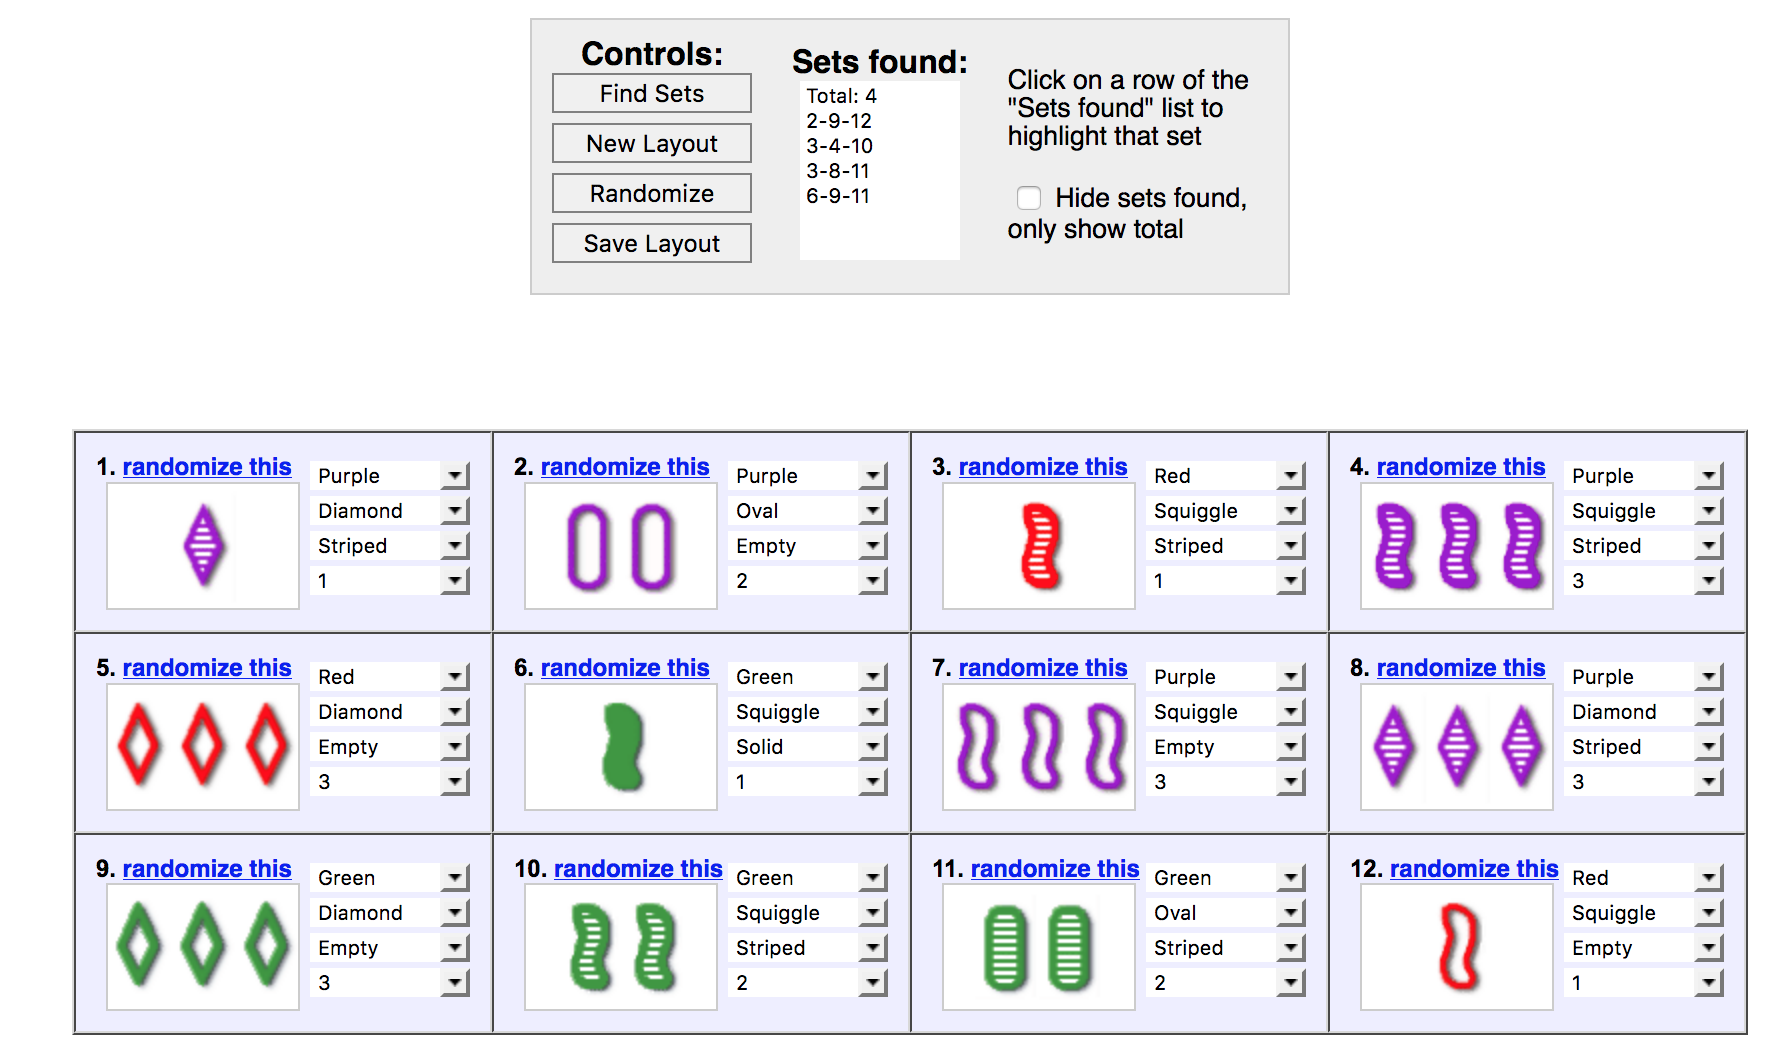
\includegraphics[width=\linewidth]{nolte.png}
\caption{Javascript SET Game Solver by Steve Nolte}
\label{fig:nolteUI}
\end{minipage}
\end{figure}


Some solvers even employ image processing to identify sets ~\cite{jorquera}. These more advanced programs are able to parse the cards from an image using computer vision and determine sets without a user inputting the cards manually. Again, this solver only supports use for one iteration of the game and will need to be updated manually to load in the new cards when the sets have been removed. All these solvers are constrained to have four properties and three values as they only apply to the original Game of Set and cannot be used for a generalized version. Moreover, all these solvers restrict their mechanism to the brute force solution. They iteratively check all possible combinations of cards to determine satisfying sets.


\section{Approach}

\subsection{SMT Solver}
Satisfiability modulo theories (SMT) are efficient solvers for constraint satisfaction problems (CSP). CSP problems arise in many areas from software verification to graph problems, and need an efficient solver to determine whether the variables and constraints are satisfiable. The most basic CSP problem is propositional satisfiability (SAT), which takes in a logical formula of boolean variables and outputs whether it is possible to satisfy the formula assigning the variables to either true or false. SMT solvers provide a more natural and richer language to encode the formula. For example, it is possible to use variables that are integers or real numbers and the constraints can be arithmetic constraints rather than a pure logical formula. The SMT solver will output whether the set of constraints can be satisfied with some assignment of the variables and can output these variables if satisfied. The basis for these SMT solvers is the use of an approach called systematic search. The search space is represented as a tree with each branch representing an assignment of a variable. The Davis-Putnam-Logemann-Loveland (DPLL) algorithm is used to efficiently search this space, and speedups can be gained by restricting this search tree as much as possible to reduce the number of branches that the algorithm must traverse ~\cite{SMTbackground}.

Generalizing the Game of Set has been done academically, but no practical solution to locate sets exists. My first implementation to solve this problem is through a reduction to SMT. SMT solvers are an efficient solver in practice for an NP-Complete problem, and I leverage this speed to solve the generalized Game of Set. Below is my reduction to SMT from the Game of Set to verify and find whether a set exists in a given board with $v$ values and $p$ properties.


\subsection{Reduction to SMT}

\subsubsection{Set Up}

There exists $v*p$ cards forming a starting board $B$, but in general, there will be $n$ cards on a board at any moment. These cards can be represented as vectors where all entries $b_{i,j} \in \{0,1, ... , v-1\}$:

\begin{align}
    B &= \begin{bmatrix}
           b_{1,1} \\
           b_{1,2} \\
           \vdots \\
           b_{1,p}
         \end{bmatrix}
         \begin{bmatrix}
           b_{2,1} \\
           b_{2,2} \\
           \vdots \\
           b_{2,p}
         \end{bmatrix} ... 
          \begin{bmatrix}
           b_{n,1} \\
           b_{n,2} \\
           \vdots \\
           b_{n,p}
         \end{bmatrix}
  \end{align}
  
The SMT Solver will then attempt to find a set of $v$ cards, labelled as $K$. The satisfying set can be denoted as vectors where $k_{i,j} \in \{0,1, ... , v-1\}$:

\begin{align}
    K &= \begin{bmatrix}
           k_{1,1} \\
           k_{1,2} \\
           \vdots \\
           k_{1,p}
         \end{bmatrix}
         \begin{bmatrix}
           k_{2,1} \\
           k_{2,2} \\
           \vdots \\
           k_{2,p}
         \end{bmatrix} ... 
          \begin{bmatrix}
           k_{v,1} \\
           k_{v,2} \\
           \vdots \\
           k_{v,p}
         \end{bmatrix}
  \end{align}

\subsubsection{All Different or All Same Constraint} The first set of constraints will only be satisfied when the cards found in $K$ represent a set, where for all properties, they have either the same or all different value. This constraint can be written as two cases for each property of the cards:

\textbf{The values are all the same for a given property i:} 
\begin{align}
	(k_{1,i} = k_{2,i}) \wedge (k_{2,i} = k_{3,i}) \wedge ... \wedge (k_{v-1,i} = k_{v,i})
\end{align}
\begin{align}
	\bigwedge \limits_{m=1}^{v-1} k_{m,i} = k_{m+1,i}
\end{align}

\textbf{The values are all different for a given property i:}
\begin{multline}
	((k_{1,i} \neq k_{2,i}) \wedge (k_{1,i} \neq k_{3,i}) \wedge ... \wedge (k_{1,i} \neq k_{v,i})) \\
	 \wedge ((k_{2,i} \neq k_{3,i}) \wedge (k_{2,i} \neq k_{4,i}) \wedge ... \wedge (k_{2,i} \neq k_{v,i})) \wedge 
	 ... \wedge (k_{v-1,i} \neq k_{v,i})
\end{multline}

\begin{align}
	\bigwedge \limits_{m=1}^{v-1}  \bigwedge \limits_{j = m+1}^{v} k_{m,i} \neq k_{j,i}
\end{align}


Therefore, we can write more concisely that for all properties of the cards, the values must all be the same or all different:

\begin{align}
	\bigwedge \limits_{i=1}^{p}  \left(  \left( \bigwedge \limits_{m=1}^{v-1}  \bigwedge \limits_{j = m+1}^{v} k_{m,i} \neq k_{j,i} \right)  \bigvee  	 \left(  \bigwedge \limits_{m=1}^{v-1} k_{m,i} = k_{m+1,i} \right) \right)
\end{align}


\subsubsection{The Cards Must Be From The Board}

The second set of constraints is that the cards selected in the set $K$ must all be from the board $B$, which is of size $n$. This constraint can be encoded into the SMT solver as:

A given card $i$ from $K$ must be from the board $B$:
\begin{multline}
	((k_{i,1} = b_{1,1}) \wedge (k_{i,2} = b_{1,2}) \wedge ... \wedge (k_{i,p} = b_{1,p})) \vee \\
	 ((k_{i,1} = b_{2,1}) \wedge (k_{i,2} = b_{2,2}) \wedge ... \wedge (k_{i,p} = b_{2,p}))  \vee ... \vee \\ ((k_{i,1} = b_{n,1}) \wedge (k_{i,2} = b_{n,2}) \wedge ... \wedge (k_{i,p} = b_{n,p})) 
\end{multline}

Therefore, all cards $i \in K$ must be from the board $B$:
 
\begin{align}
	\bigwedge \limits_{i=1}^{v}  \left( \bigvee \limits_{j = 1}^{n}  \left( \bigwedge \limits_{m=1}^{p}  k_{i,m} = b_{j,m}\right) \right)
\end{align}

\subsubsection{All Distinct Cards}

We constrain the possible cards in the set to be from $B$, but this includes using duplicate cards. A possible set could be $v$ of the exact same card and would satisfy the above constraints but does not represent a real set in the game. Therefore, the cards selected to be in $K$ must all be distinct cards. The cards of a set are considered all distinct if for any two cards, they have at least one property that has a differing value. The constraint can be written as:


%%%% possibly rewrite this better such that for a given card i make sure that the cards above it (ie. j = i+1) are all totally distinct
%%% and then more concisely can write that for all it would be better... pick one

A given card, $i$, differs with respect to at least one property compared to all cards after $i:$

\begin{multline}
	((k_{i,1} \neq k_{i+1,1}) \vee (k_{i,2} \neq k_{i+1,2}) \vee ... \vee (k_{i,p} \neq k_{i+1,p}))  \wedge \\
	((k_{i,1} \neq k_{i+2,1}) \vee (k_{i,2} \neq k_{i+2,2}) \vee ... \vee (k_{i,p} \neq k_{i+2,p}))  \wedge ... \wedge \\ 
	((k_{i,1} \neq k_{v,1}) \vee (k_{i,2} \neq k_{v,2}) \vee ... \vee (k_{i,p} \neq k_{v,p})) 
\end{multline}

Written more succinctly:


%\begin{multline}
%	((k_{1,1} \neq k_{2,1}) \vee (k_{1,2} \neq k_{2,2}) \vee ... \vee (k_{1,p} \neq k_{2,p}))  \wedge \\
%	((k_{1,1} \neq k_{3,1}) \vee (k_{1,2} \neq k_{3,2}) \vee ... \vee (k_{1,p} \neq k_{3,p}))  \wedge ... \wedge \\ 
%	((k_{1,1} \neq k_{v,1}) \vee (k_{1,2} \neq k_{v,2}) \vee ... \vee (k_{1,p} \neq k_{v,p})) \wedge \\
%	((k_{2,1} \neq k_{3,1}) \vee (k_{2,2} \neq k_{3,2}) \vee ... \vee (k_{2,p} \neq k_{3,p})) \wedge  ... \wedge \\ 
%	((k_{2,1} \neq k_{v,1}) \vee (k_{2,2} \neq k_{v,2}) \vee ... \vee (k_{2,p} \neq k_{v,p})) \wedge ... \wedge \\
%	((k_{v-1,1} \neq k_{v,1}) \vee (k_{v-1,2} \neq k_{v,2}) \vee ... \vee (k_{v-1,p} \neq k_{v,p})) 
%\end{multline}



\begin{align}
	\bigwedge \limits_{i=1}^{v-1}   \left( \bigwedge \limits_{j=i+1}^{v}   \left( \bigvee \limits_{m = 1}^{p} k_{i,m} \neq k_{j,m} \right)  \right)
\end{align}

\subsubsection {Symmetry Breaking}

% initial way to do it by sorted!
The first constraint I used to break the symmetry of the search space is for every possible set, the cards need to be in sorted order by their first property, but if the values are all the same, then sorted by the second property, and so forth if the cards in the set have equivalent value for a given property. This symmetry breaking constraint is labelled as the relative sorted constraint and can be encoded as follows: 

\begin{multline}
	(k_{1,1} \leq k_{2,1} \leq ... \leq k_{v,1}) \wedge (   (k_{1,2} \leq k_{2,2} \leq ... \leq k_{v,2})  \vee \neg (k_{1,1} = k_{2,1} = ... = k_{v,1})) \\
	\wedge (   (k_{1,3} \leq k_{2,3} \leq ... \leq k_{v,3})  \vee \neg (k_{1,2} = k_{2,2} = ... = k_{v,2}) \vee \neg (k_{1,1} = k_{2,1} = ... = k_{v,1})) \\
	\wedge ... \wedge (   (k_{1,p} \leq k_{2,p} \leq ... \leq k_{v,p})  \vee \neg (k_{1,p-1} = k_{2,p-1} = ... = k_{v,p-1}) \vee ... \vee \neg (k_{1,1} = k_{2,1} = ... = k_{v,1}))
\end{multline}

Written more compactly:

\begin{align}
	\bigwedge \limits_{i=1}^{p}   \left(  (k_{1,i} \leq k_{2,i} \leq ... \leq k_{v,i}) \bigvee \limits_{j=1}^{i-1}  \left( \neg (k_{1,j} = k_{2,j} = ... = k_{v,j})  \right)   \right)
\end{align}


% other way... CHECK SPEEDS!!!

The above symmetry breaking constraint condenses the search tree to a certain degree, but still searches some branches unnecessarily. For example, if a set is cards [0,1,2], the solver could potentially first check [1,2], then add 0 at the end when it would finally realize that this is not sorted. The algorithm would waste time as we know the first card must have the lowest value, 0, to be considered sorted. Therefore, we can rigidly constrain it such that for the first property in which they differ, the first card's value must be 0, the second card's 1, and so forth. This restricts the search space further. This symmetry breaking constraint is labelled as the rigid sorted constraint and can be encoded as follows:

\begin{multline}
	(k_{1,1} = 0, k_{2,1} = 1 , ... , k_{v,1} = v-1) \wedge (   (k_{1,2} = 0, k_{2,2} = 1, ... , k_{v,2} = v-1)  \vee \neg (k_{1,1} = k_{2,1} = ... = k_{v,1})) \\
	\wedge (   (k_{1,3} = 0,  k_{2,3} = 1,  ... , k_{v,3} = v-1)  \vee \neg (k_{1,2} = k_{2,2} = ... = k_{v,2}) \vee \neg (k_{1,1} = k_{2,1} = ... = k_{v,1})) \\
	\wedge ... \wedge (   (k_{1,p} = 0 , k_{2,p} =1,  ... , k_{v,p} = v-1)  \vee \neg (k_{1,p-1} = k_{2,p-1} = ... = k_{v,p-1}) \vee ... \vee \neg (k_{1,1} = k_{2,1} = ... = k_{v,1}))
\end{multline}

Written more compactly:

\begin{align}
	\bigwedge \limits_{i=1}^{p}   \left(  (k_{1,i} = 0, k_{2,i} =1,  ... , k_{v,i} = v-1) \bigvee \limits_{j=1}^{i-1}  \left( \neg (k_{1,j} = k_{2,j} = ... = k_{v,j})  \right)   \right)
\end{align}

These two strategies are different and I will explore the relative effectiveness of both in the implementation section.

By building these four constraints (7, 9, 11, and 13 or 15) from a given board, we can reduce finding an arbitrary set to SMT and use a solver to locate a set efficiently. 

\subsubsection{Update Functions} 
The solver to find sets must also support two update functions. The first update function of removing cards can be easily encoded into the SMT constraints. Let set $V$ be an arbitrary set that was located by the SMT solver. We can add new constraints such that the new set to be found cannot be equal to any of the cards found in $V$, where $V$ contains $v$ cards. Again, to be a distinct card, at least one property must be differing. 

A given card $i$ from $K$ must not be equivalent to a card in $V$:

\begin{multline}
	((k_{i,1} \neq v_{1,1}) \vee (k_{i,2} \neq v_{1,2}) \vee ... \vee (k_{i,p} \neq v_{1,p})) \wedge \\
	 ((k_{i,1} \neq v_{2,1}) \vee (k_{i,2} \neq v_{2,2}) \vee ... \vee (k_{i,p} \neq v_{2,p}))  \wedge ... \wedge \\ ((k_{i,1} \neq v_{v,1}) \vee (k_{i,2} \neq v_{v,2}) \vee ... \vee (k_{i,p} \neq v_{v,p})) 
\end{multline}

All cards $i \in K$ must not be equivalent to a card in $V$:

\begin{align}
	\bigwedge \limits_{i=1}^{v}   \left( \bigwedge \limits_{j=1}^{v}  \left( \bigvee \limits_{m = 1}^{p} k_{i,m} \neq v_{j,m} \right)   \right)
\end{align}




For the second update function in which new cards may be added to the deck, we will need to create a new set of constraints (7, 9, 11, and 13 or 15) from above to locate a complete set. Therefore, this is represents a full reduction to SMT from the Game of Set. 

However, in this generalized game for some values of $p$ and $v$, it might not locate a set within reasonable time in practice if we consider the the poly-time transformation and the fact that it needs to recalculate a set every time new cards are added, not using information from previous rounds.

\subsection{Dynamic Algorithm}

The dynamic algorithm approach uses previous knowledge of the board between draws to quickly discover sets. This approach will be useful because of the nature of the game's changing probabilities as it is played. It has been shown that on an initial layout of the game with 12 cards, the ratio of games in which there exists a Set to those that do not contain a set, is 29:1. But as the game plays on, the ratio drops to 15:1, a 50\% less chance of finding a set. For 15 cards, the ratio drops to 4\% of its original ratio as the game is played ~\cite{norvig}. Therefore, as the game is iteratively played in which sets are taken out, the game becomes immensely harder. Finding a high number of sets $n$ will be hard if many cards must be drawn. Remembering partial sets across draws can greatly speed up the algorithm if we know that it will take many draws to find complete sets. I will also employ a similar symmetry breaking constraint from the SMT solver for the dynamic algorithm to create a faster algorithm, as instead of storing all possible permutations of a partial set, I will only store the one set that a permutation will condense to by keeping each partial set sorted. The dynamic algorithm solver I build should be able to beat the SMT solver for some cases of $v,p,$ and $n$ considering the added difficulty of the game as we add new cards.

\section{Implementation}

The randomizer to create cards and solvers were all written in Python. Considering Python's lightweight feel and ease of iterating over all variables in a list, it is the natural choice to represent a deck and board of cards, where we must iterate over them regularly. Therefore, I selected to use Python as the coding language for the entirety of the project. 


\subsection{Randomizer}

The randomization algorithm for creating a randomized deck is very important in terms of creating real gameplay. The algorithm must uniformly distribute all of the cards ($v^p$) initially so that no solver can have an unfair advantage knowing what cards are more likely to appear. I used the Random library in Python to generate cards. To ensure the cards drawn were unbiased, I employed the use of a modified version of Fisher Yates Shuffle. Fisher Yates Shuffle works by iteratively picking random indices from a finite sequence and produces an unbiased permutation \cite{fisher}. To convert the algorithm for use on a deck, I used rejection sampling to determine new cards to add to the board. I created a card by randomly generating a string of length $p$ and, for each property, randomly generating a value from $0$ to $v-1$. If the card was not in the board already and not in the removed cards set (ie. part of a set that was already found), I added it. If it was a duplicate of a card I had already seen, I generated another card until I have created $v*p$ cards that are all distinct. Since the algorithm uses a randomized strategy but will always produce a board whose cards are all distinct and from the deck with equal probabilities, it is an example of a Las Vegas algorithm. To support the update function of removing cards, I appended those cards to a set of removed cards that cannot be used for new cards. Therefore, when $v$ new cards are to be added, I generated $v$ new random cards through the above algorithm to be added to the board. This yields a randomized $v*p$ starting boards and unbiased drawing of $v$ cards from the deck.

To confirm that this in fact created random initial boards and $v$ new cards, I graphed the distribution of the beginning board for $1000$ trials with two different cases, $v=4$ and $p=3$ and $v=5$ and $p=4$. I then used numpy and matplotlib to count all the occurrences of each card and graph them as a histogram. In Figures~\ref{fig:init1}  and~\ref{fig:init2}, we can see that in both cases (3 properties, 4 values and 4 properties, 5 values), the distribution of cards that were initially selected to be on the board form a uniform distribution over 10,000 trials.

\begin{figure}[htbb]
\begin{minipage}[b]{0.5\linewidth}
\centering
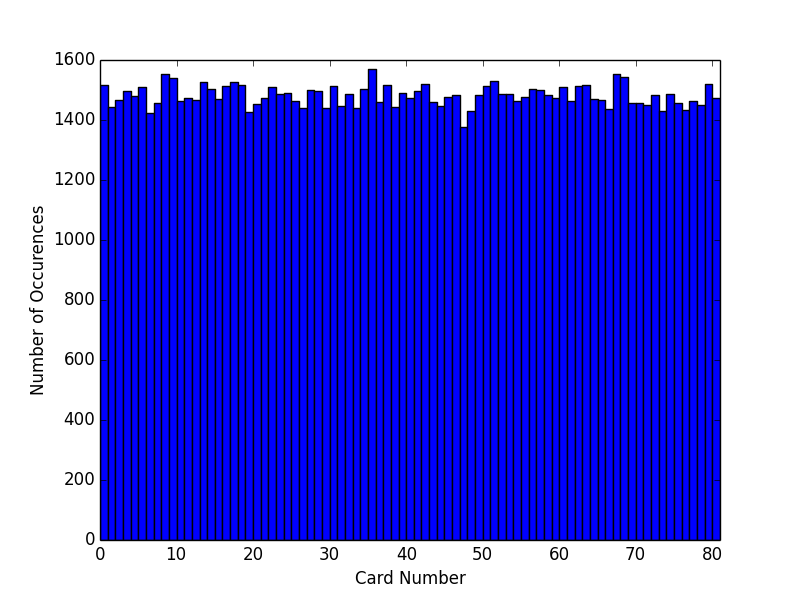
\includegraphics[width=.75\linewidth]{3p4v10000Init.png}
\caption{3 properties, 4 values, 10,000 trials Initial Board Distribution}
\label{fig:init1}
\end{minipage}
\hspace{0.5cm}
\begin{minipage}[b]{0.5\linewidth}
\centering
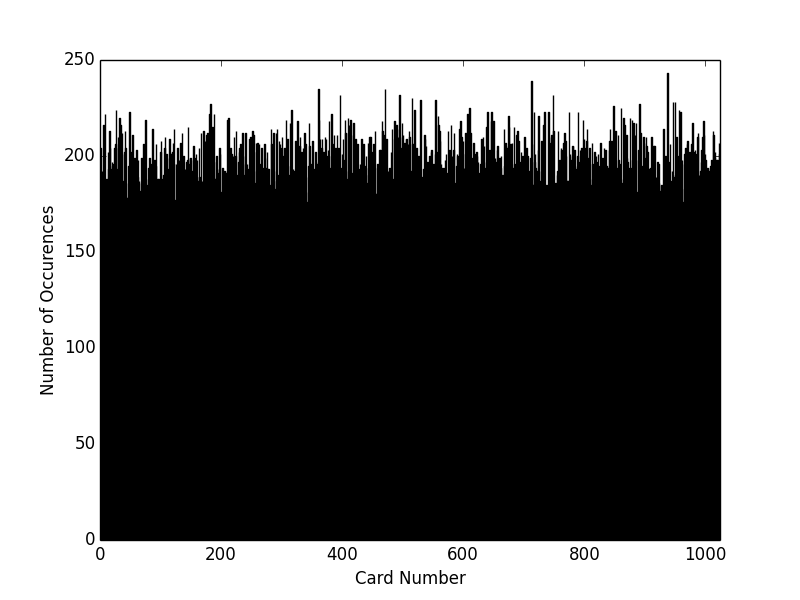
\includegraphics[width=.75\linewidth]{4p5v10000Init.png}
\caption{4 properties, 5 values, 10,000 trials Initial Board Distribution}
\label{fig:init2}
\end{minipage}
\begin{minipage}[b]{0.5\linewidth}
\centering
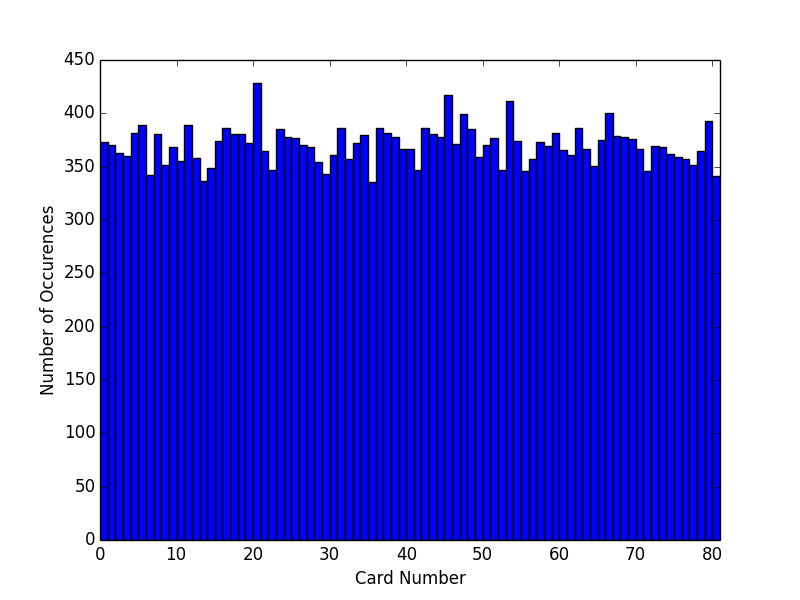
\includegraphics[width=.75\linewidth]{3p4v10000Draw.png}
\caption{3 properties, 4 values, 10,000 trials Distribution of $4$ New Cards Drawn}
\label{fig:draw1}
\end{minipage}
\hspace{0.5cm}
\begin{minipage}[b]{0.5\linewidth}
\centering
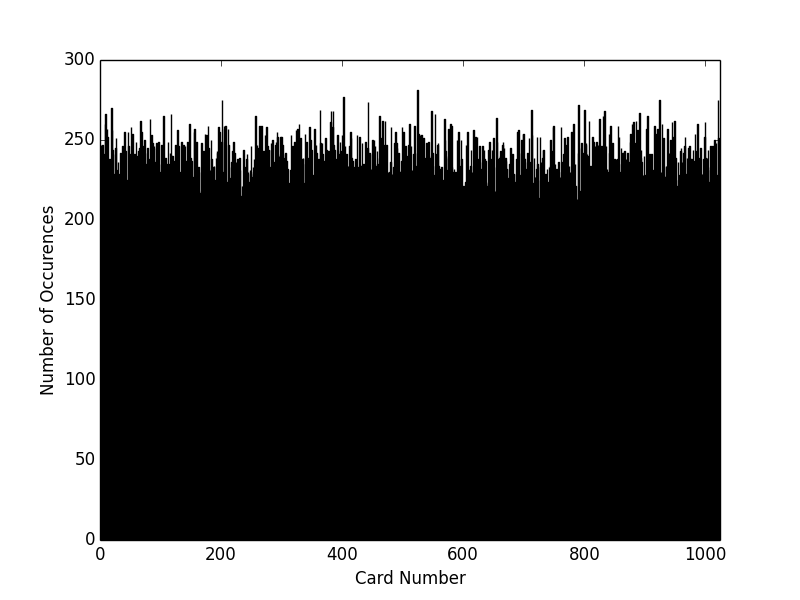
\includegraphics[width=.75\linewidth]{4p5v10000Draw.png}
\caption{4 properties, 5 values, 10,000 trials Distribution of $5$ New Cards Drawn}
\label{fig:draw2}
\end{minipage}
\end{figure}


The distribution of cards drawn (excluding the starting board and only counting the $v$ new cards drawn) also forms a uniform distribution as can be seen in Figures~\ref{fig:draw1}  and~\ref{fig:draw2}, when the boards have 3 properties, 4 values and 4 properties, 5 values over 10,000 trials. Therefore, this confirms that the implementation of the Fisher Yates shuffle in creating a perfectly random board and draws was successful. 


\subsection{Brute Force Implementation}

As a naive implementation, I created a brute force solution that tests all possible combinations of $v$ cards till a set is found and returns this set. A maximum number of ${v*p}\choose{v}$ possible sets will have to be examined before a set is found. This can be carried out $n$ times to find $n$ sets and therefore does not build on any previous knowledge, completely checking all possible sets each iteration, though it may have checked the possible set in a previous search. Though not optimized in any way, the brute force implementation provides a benchmark algorithm to compare the SMT based and dynamic algorithm against. 

\subsection{SMT Solver Implementation}


\subsubsection{Z3}
I used Z3, a high performance theorem prover created by Microsoft Research. The software allows me to easily create variables and constraints in Python. Each card that needs to be found represents $p$ variables, or $v*p$ total variables for all cards. I coded the above constraints in Z3 and if the SMT solver outputs "sat," then we know there exists a satisfying set of assignments for the variables with these constraints. Therefore, this satisfying assignments represents the $v$ cards that compose a set. If the SMT solver is "unsat," then there exists no satisfying assignment and more cards must be drawn to find a set. 

\subsubsection{Delayed Deletion Optimization}

To optimize the SMT Solver implementation, I queue up the set to be removed and add constraint 17 (a satisfying set cannot include any card that was found to be part of a set) to run through the SMT Solver again to find another set to be removed in case there exists many sets already on the starting board. Once the SMT Solver no longer says a set exists, I then add $v$ new cards to hopefully create a new set. I will only do this once no set exists on the board after removing many cards to provide marginal speedup to the program as the solver will not have to rebuild many constraints every time a set is found. Once no sets exist on the board and I draw the corresponding number of cards, I rebuild the constraints and run the SMT solver to hopefully find another set of cards. 


\subsubsection{Constraining the Domain Optimization}

The SMT solver iteratively searches for a solution through a search tree, attempting to constrain the domain for each variable until a satisfying assignment has been discovered, a process called forward checking, or all the possible assignments have been exhausted and the constraints cannot be satisfied \cite{search_from_AI}. In this game, the SMT solver will be forced to check every permutation of cards for a set, when in reality, all permutations of a given set are equivalent because order does not matter in a set of cards to satisfy the constraints. To break this symmetry for multiple sets, constraint 13 and 15 enforce that the cards in a set are in sorted order (ie. by the first property or if all equal then by the second property and so forth for all properties) and constrains the domain of each variable. This will break the symmetry in the encoding and speed up the process of the SMT solver, as the SMT solver will not need to search branches of its search tree that are duplicates of another branch. 

\subsection{Dynamic Algorithm Implementation}

The dynamic algorithm approach hinges on the tradeoff between memory and speed. The brute force solution does not need to keep track of partial sets and spends time iterating over all combos as fast possible. The dynamic algorithm is on the other side of the spectrum and utilizes much more space, recording all possible sets that can be quickly completed, but does so in hopes for a benefit in overall speed. 

The dynamic algorithm's main speedup is in the way that it creates a list of partial sets and a dictionary mapping the missing card to an almost complete partial set, in the hopes that it can quickly finish these sets when new cards are drawn. Outlined below is the general algorithm. 

\subsubsection{Set Up}

To create all partial sets, the dynamic approach begins similarly to the brute force solution. When the board is created, the solver will initially create partial sets for all ${v*p}\choose{2}$ combinations of two cards using Python's built in itertools library since a possible set can be determined by any two cards (ie. if the first two cards have the same value for a given property, the satisfying cards must have the same value for that property or if different than all the values need to be different). These two card partial sets will be the basis for creating larger partial sets and will ensure that all combinations of cards are checked to complete a set. I also include a symmetry breaking constraint, identical to the optimal SMT solver of retaining only sorted sets, as adding in cards to a partial set will create many duplicate partial sets. As an example of how this condenses the space of partial lists consider this example: Starting with partial sets [0,1] and [1,2], when I add 2 to the first set and 0 to the second, they will both yield set [0,1,2]. However, these are identical partial sets and would cause the search space to expand unnecessarily.  Therefore, I keep the partial sets sorted at all times (by saying that the first property for which they differ, they must be in sorted order), and when I add a new partial set to the partial set list I check whether it already exists, thereby not creating duplicates in this partial set list.

\subsubsection{Partial Set List and Quick Complete Dictionary Creation}

For each partial set, the algorithm determines which cards can be added to the partial set from the board that satisfy the constraints that for each property, the values are either the same or all different and must not be in the set of cards that we flag as unusable cards as they have been used to complete a set in a previous iteration. 

If a card can be added, I copy the given partial set and add the new card to it (if I added card 2 to a set [0, 1], I append [0,1,2] to the partial set list and keep [0,1] just in case a card I draw later will determine a whole new set), creating a  new partial set that is again sorted and verified that it is not in the partial set list already. Then, I append it at the end of the partial set list. This practice also ensures that new partial sets I append will not interfere with any previous sets. I must keep the original set because depending on how new cards are drawn, this stub set can be satisfied differently (ie. I can add [0,1,3] while not interfering with [0,1,2] if 3 and 2 conflict with each other as [0,1] is left after matching to 2 so it can be matched with 3). By adding the cards incrementally, if it does happen that both cards satisfy the set, (ie. [0,1,2,3] is a set), then when I add the last card to the set it will see that it already exists in the partial set list by the symmetry breaking constraint and will delete one of the partial sets.

When I add cards to a partial set, its size can be in one of two cases:

\textbf{Case 1: Size $v$:} If the partial set is completely full and at size $v$, then the partial set is a complete satisfying set and can therefore be queued as a found set. These cards will also be queued up as cards that will need to be deleted from the partial sets and board and cannot be used to complete other partial sets.

\textbf{Case 2: Otherwise:} This partial set is missing more than one card. Therefore, we must append this new set to the end of the partial sets as this is a partial set that can be satisfied by adding new cards from the board. Python for loop construction is also very powerful and supports iterating over an expanding list. Therefore, it will reach all partial sets, even if added after the initialization of the for loop. 

At the end of iterating through all partial sets, I will have had attempted to add all possible cards to all possible sets. Therefore, no cards could be added to any partial set without violating the satisfying constraint. We will have found all sets that could have been finished in the given board. Now, I iterate over all partial sets to see which sets are almost completed (size $v-1$). If they are missing one card, I create the quick complete data structure. The last card can be wholly determined by the cards currently in the set as the value will be the same if the set has the same value for a given property and if they are all different then it will be the last missing value. I add to the dictionary the missing card mapped to the partial set it completes.

\subsubsection{Quick Complete Upon Drawing Cards}

When more sets are needed to be found than exist on the board, new cards must be drawn to create an opportunity for more sets. When these $v$ new cards are drawn, the dynamic algorithm will use its quick complete dictionary to quickly search to see if any of the $v$ cards drawn satisfy any of the partial sets that are missing one card. If they complete a partial set, the dictionary will delete the card from its table, append it to the partial set it completes, and add it to the queue of found cards. As we iterate through, it is possible that the cards used in one of these quick completed sets could be used for another completed set and therefore we need to ensure that any card was not used to complete a previous set. 

After we have completed all of the partial sets we could have with the new drawn cards, we must create new stub partial sets from these new cards. I create combinations over all new cards and all cards currently on the board (ie. if there are $v'$ new cards left after quick completing and $n'$ cards on the board, I create $v'*(n'+v'-1)$ new stub partial sets to be added to the partial sets list). With these new partial sets appended, the program then reruns the algorithm described above in Partial Set List and Quick Complete Dictionary Creation to find new sets and create the appropriate data structures for future iterations. 

\subsubsection{Deletion Bookkeeping}

After both of the above steps, we need to ensure that any found set's cards are appropriately removed from the partial sets. Therefore, I iterate over all partial sets and see if any of them contain a card that was used to complete a set. If it does, I delete the entire partial set. This ensures that we will not be harboring any duplicate partial sets as we retain all partial sets as well. For example, if the card 3 needed to be deleted, we would delete the entire partial set [0,1,2,3]. We can delete the entire set as we retain the partial set [0,1,2] by the above step of the algorithm. Therefore, we can remove all partial sets that contain cards that were used to create a completed set.

I also iterate over the quick complete dictionary and if any of the almost completed partial sets contain a card we are removing, I delete that appropriate entry from the dictionary as it is now missing more than one card which was the criteria to be included in the quick complete dictionary. Once we have deleted the cards from the appropriate data structures, we can iteratively continue these steps until $n$ sets have been found. 

\subsubsection{Finding a Set}

When the dynamic algorithm does find a set, either through quick complete or while appending all satisfying cards to a partial set, it checks whether it has found $n$ sets. If it has, it will immediately return and therefore will not have to waste time constructing all of the partial sets for subsequent iterations if it had found the threshold of $n$ sets. This will speed up the final iteration as we will not build the complementary data structures unnecessarily. 

\subsection{Testing}

For both of these implementation, I created testing infrastructure to ensure that the sets found by the solvers are indeed sets, and that the algorithm correctly removed the sets from the board. 

\subsubsection{Testing Satisfying Set}

To confirm that for all properties the cards from the set have either the same value or all different value, I iterated over all properties and check whether when I put the values from each property into a set data structure that the length of the set was either 1, meaning that all the values were the same, or of length $v$, meaning all values were distinct elements. 

To check that all the cards must be from the board, I had to store all iterations of the board, as new cards could be added and sets would be removed. Therefore, I used a set data structure to store all the cards, and updated this set as new cards were added to the board. Finally, I iterated over each set found and checked that it was included in the board at some point and therefore meant it was taken from the board. 

To confirm that the last constraint of all distinct cards was satisfied for each possible set, I asserted that the length of the set was equivalent to the length of the set when converted into a set data structure. Therefore, if they are equal, all elements in the set are distinct.

Finally, the solver has to handle finding many sets, and to ensure that the solver does not find the same set $n$ times, I assert that when converted to a long list of cards that make up all $n$ sets found, that the length of this list converted to a set data structure should be the same as the length of the long list. Therefore, it would show that all $n*v$ cards are all distinct. 

\subsubsection{Testing Correct Deletion}

The constraints created for the SMT solver also relies on the fact that the cards from a satisfying set must be deleted from the board at some point. Therefore, as a check to ensure that the corresponding cards were deleted from the board, I iterated over all cards and asserted that all the cards found as part of sets were no longer part of the board at termination of the program. This is a good double check to ensure that SMT solver is functioning properly, because the SMT hinges on the fact that cards that can no longer be used are deleted from the board before rebuilding the constraints. This is also important for the dynamic algorithm and brute force implementation because they must output the correct board as well after finding $n$ sets. At termination, we iterate over all cards found as being part of sets and assert that they are no longer part of the board.

\section{Results and Evaluation}

\subsection{Timing Tests}

To test the relative effectiveness of the three implementations, I divided the testing into three cases to see how the implementations functioned on a variety of test cases. Since there are three variables to change, number of values, properties, and sets to find, I vary one of them and keep the other two constant. This creates a total of three overarching categories that can be broken down further as the two constant variables can take on different values. 

To accurately test the timing of each solver, I utilized Python's time library to accurately test CPU time used for each of the processes. Therefore, if other processes are running in the background, they will not factor into the timing tests of these solvers. Also, only the process of creating the solver data structure and finding $n$ sets is accounted in CPU time, as creating the randomizer and verification of correct sets following finding the sets is irrelevant to the speed of the solver itself. 

To give more accurate results, the times for a given set of values, properties, and sets to find are averaged over ten trials to give one data point. Therefore, this would account for instances in which a set can be found instantly or if all combinations need to be examined to find a set, and would give a more accurate time for a test case. Also, for each of the ten trials, I test each solver with the same beginning board such that we can see how they match up directly against each other on the same board.

I again used matplotlib to graph the time trials. These graphs are composed of connected dotted lines that are color coded by solver. 


\subsection{Brute Force Inefficiency}

The brute force implementation is the solution that many solvers online employ. The brute force solution is efficient enough and fast in the case of the actual Game of Set in which there are only $3$ values and $4$ properties, even being able to beat the SMT solver and dynamic algorithm in some cases. However, as $v$, $p$, and $n$ are increased to add complexity to the problem, the brute force solution begins to take exponential time. Therefore, the brute force solution must be deleted in real timing tests between the SMT solver and dynamic algorithm to provide fair competition and not ruin the scale of the graphs. To see the inefficiency of the brute force implementation, see Figure~\ref{fig:bruteVal} as we vary the value and~\ref{fig:bruteProp} as we change the number of properties.


\begin{figure}[htbb]
\begin{minipage}[b]{0.5\linewidth}
\centering
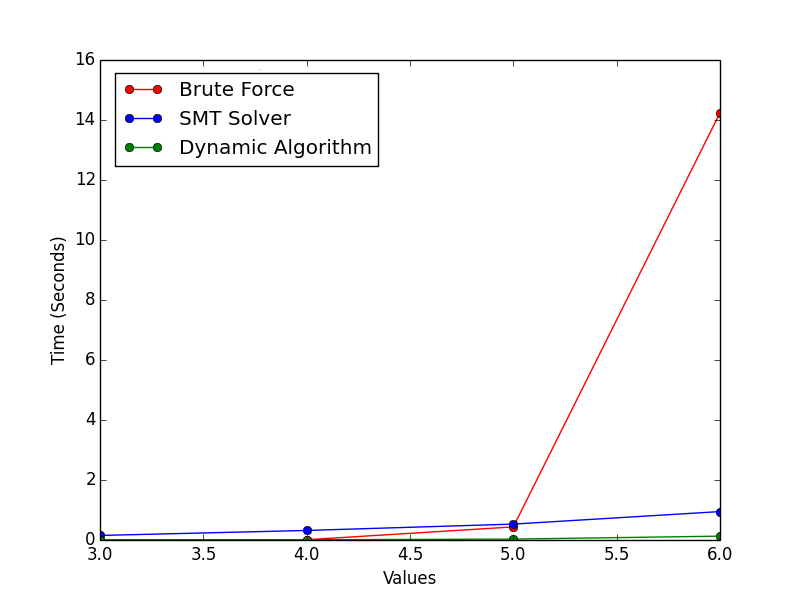
\includegraphics[width=.75\linewidth]{BADBRUTEVAL-v3456p3n5.png}
\caption{3 Properties and 5 Sets Found Varying the Number of Values}
\label{fig:bruteVal}
\end{minipage}
\hspace{0.5cm}
\begin{minipage}[b]{0.5\linewidth}
\centering
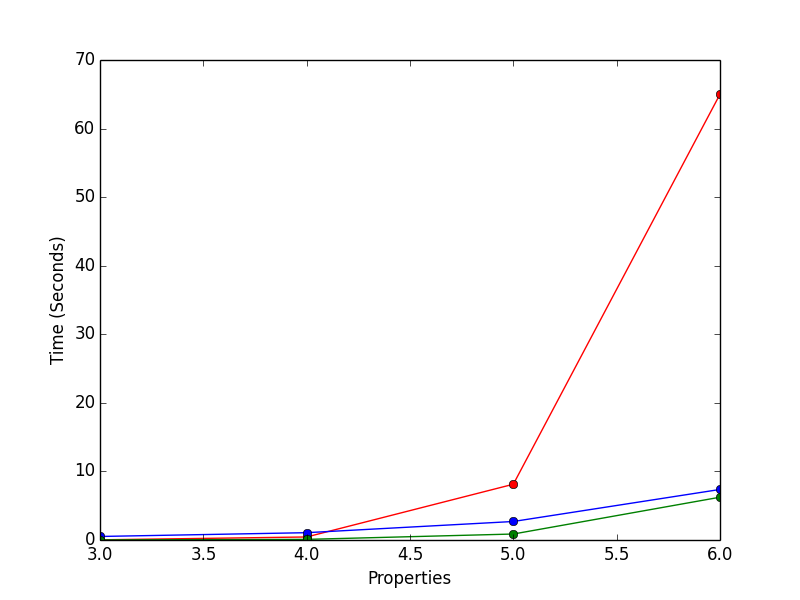
\includegraphics[width=.75\linewidth]{BADBRUTEPROP-v4p3456n10.png}
\caption{4 Values and 10 Sets Found Varying the Number of Properties}
\label{fig:bruteProp}
\end{minipage}
\end{figure}



\subsection{Comparing Symmetry Breaking Constraints}

The first symmetry breaking constraint I used dictated that for the first property in which they differed, they needed to be sorted by that property. However, this was a relative constraint and did not condense the search tree as much as possible, labelled as constraint 13 above. Therefore, I also created an alternate constraint that is more specific and rigidly dictates that for the first property in which the differ the first card's value has to be 0 and so forth, labelled as constraint 15 above. 

We can see the effect of symmetry breaking in Figure ~\ref{fig:VersusSMTVal} and ~\ref{fig:VersusSMTProp}, in which I graph the speed of the three variations of the SMT solver against each other. As the number of values of the game is increased, the no condensing SMT solver's run time blows up exponentially. We can see that the symmetry breaking constraints do provide considerable speed up for all different values. 

\begin{figure}[htbb]
\begin{minipage}[b]{0.5\linewidth}
\centering
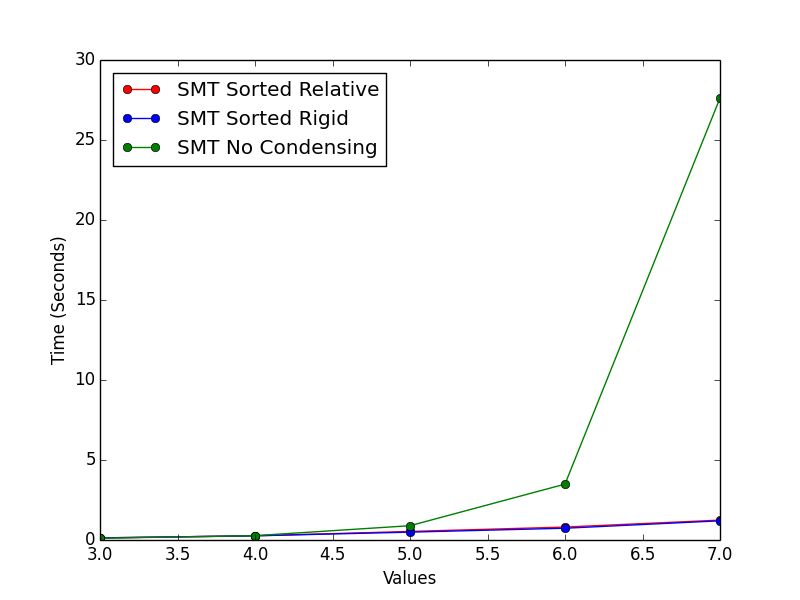
\includegraphics[width=.75\linewidth]{VersusSMTVAL-v34567p3n5.png}
\caption{3 Properties and 5 Sets Found Varying the Number of Values}
\label{fig:VersusSMTVal}
\end{minipage}
\hspace{0.5cm}
\begin{minipage}[b]{0.5\linewidth}
\centering
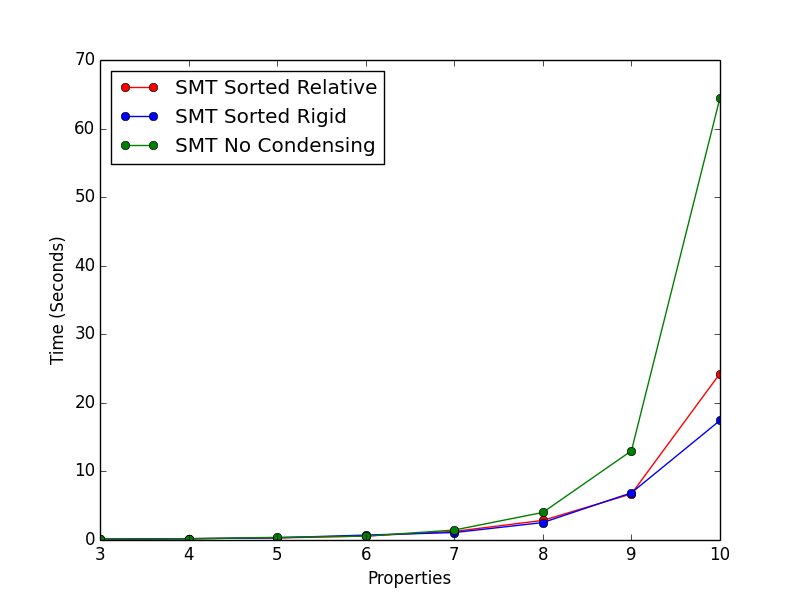
\includegraphics[width=.75\linewidth]{VersusSMTPROP-v3p345678910n5.png}
\caption{3 Values and 10 Sets Found Varying the Number of Properties}
\label{fig:VersusSMTProp}
\end{minipage}
\end{figure}

% choosing which SMT solver condesning condition to use


% now between the two of the fastest


Now, to determine which symmetry breaking constraint yields the greatest speedup, I run the two implementations against each other. As the rigidly sorted constraint condenses the search space more than the relative sorted, the speed up of adding this constraint can be seen in Figure~\ref{fig:RunoffVAL} and~\ref{fig:RunoffPROP}. In all cases, the rigid sort is marginally faster and this difference increases as the parameter increases. Therefore, for the final implementation of the SMT solver, I settled on using the rigidly sorted constraint. This is the fastest version of the SMT solver and would provide the best competitor against the dynamic algorithm.



\begin{figure}[htbb]
\begin{minipage}[b]{0.5\linewidth}
\centering
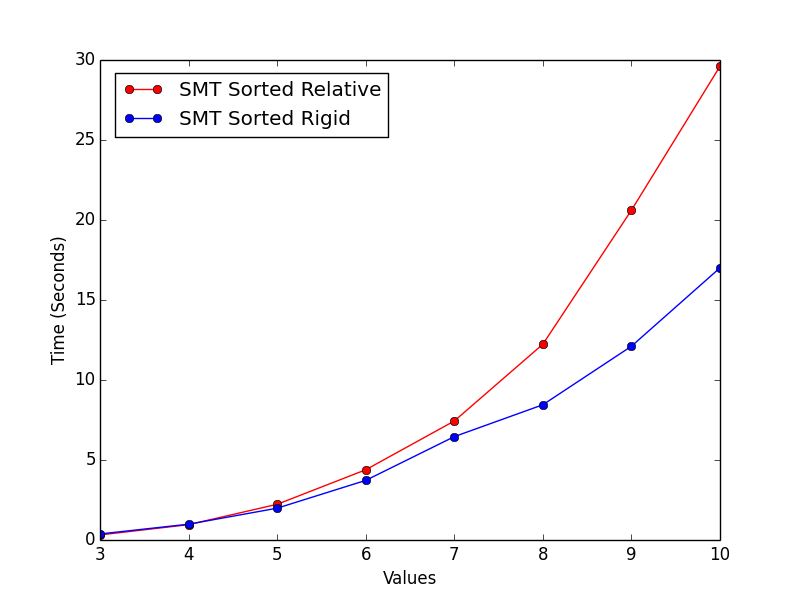
\includegraphics[width=.75\linewidth]{RunoffSMTVAL-v345678910p4n10.png}
\caption{4 Properties and 10 Sets Found Varying the Number of Values}
\label{fig:RunoffVAL}
\end{minipage}
\hspace{0.5cm}
\begin{minipage}[b]{0.5\linewidth}
\centering
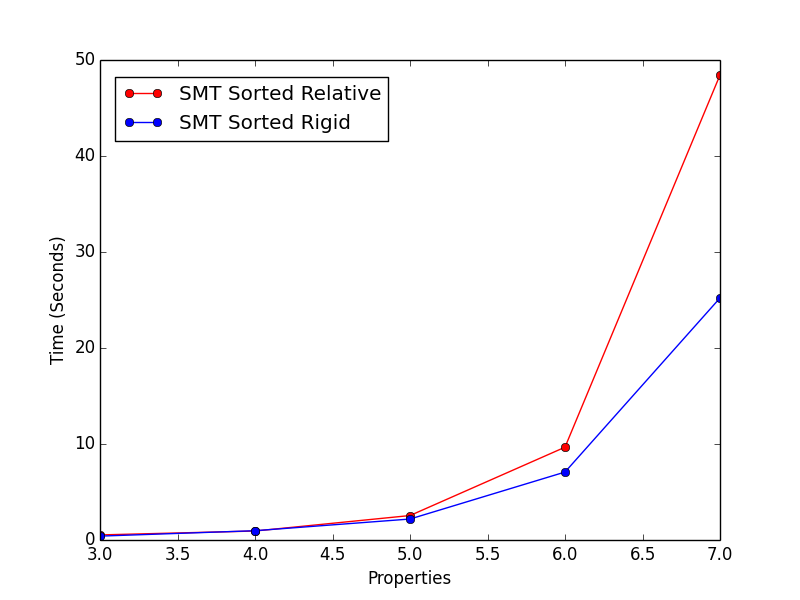
\includegraphics[width=.75\linewidth]{RunoffSMTPROP-v4p34567n10.png}
\caption{4 Values and 10 Sets Found Varying the Number of Properties}
\label{fig:RunoffPROP}
\end{minipage}
\end{figure}

\subsection{Comparing the Final Implementations of the Dynamic Algorithm and SMT Solver}

\subsection{Varying the Number of Values}

There exists a threshold for which the dynamic algorithm performs better than the SMT solver. See Figure~\ref{fig:DvSVAL}. Up until there are 5 values, the dynamic algorithm is marginally faster than the SMT solver, but once the number of values increases past 5, the time grows exponentially while the SMT solver is relatively linear. At this threshold, the dynamic algorithm takes much too long and it becomes only feasible to run the SMT solver by itself. 

The SMT solver is able to handle values as large as 10, even with 4 properties instead of 3 properties from the previous figure, while still retaining its linear growth. See Figure~\ref{fig:SMTVal}. The dynamic algorithm performs much worse because of how many more partial sets it has to store. As we increase the number of values, the dynamic algorithm will store larger partial sets because satisfying sets will be larger (of size $v$ where $v$ is the number of values). Memory usage will be higher and iterating over these sets will take more time. This explains why the dynamic algorithm grows exponentially while the SMT solver is relatively linear with respect to the number of values. 


\begin{figure}[htbb]
\begin{minipage}[b]{0.5\linewidth}
\centering
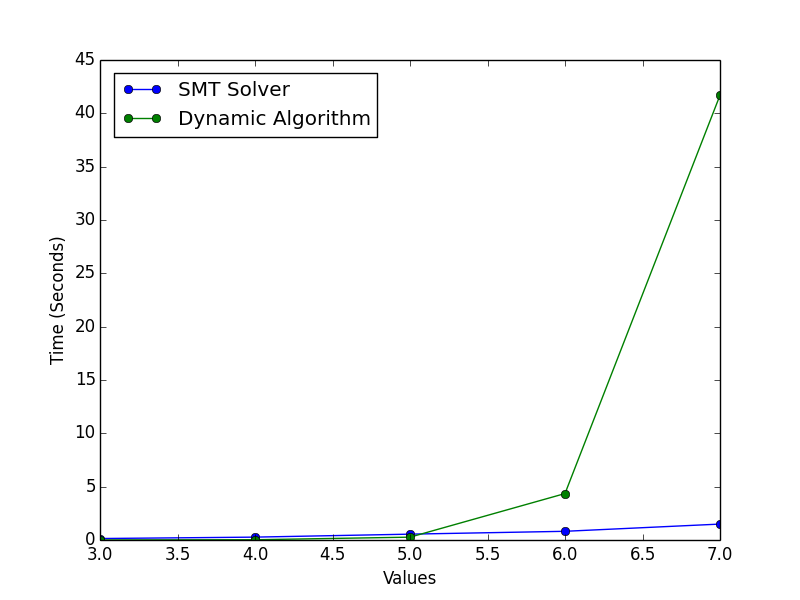
\includegraphics[width=.75\linewidth]{DvSVAL-v34567p3n5.png}
\caption{3 Properties and 5 Sets Found Varying the Number of Values}
\label{fig:DvSVAL}
\end{minipage}
\hspace{0.5cm}
\begin{minipage}[b]{0.5\linewidth}
\centering
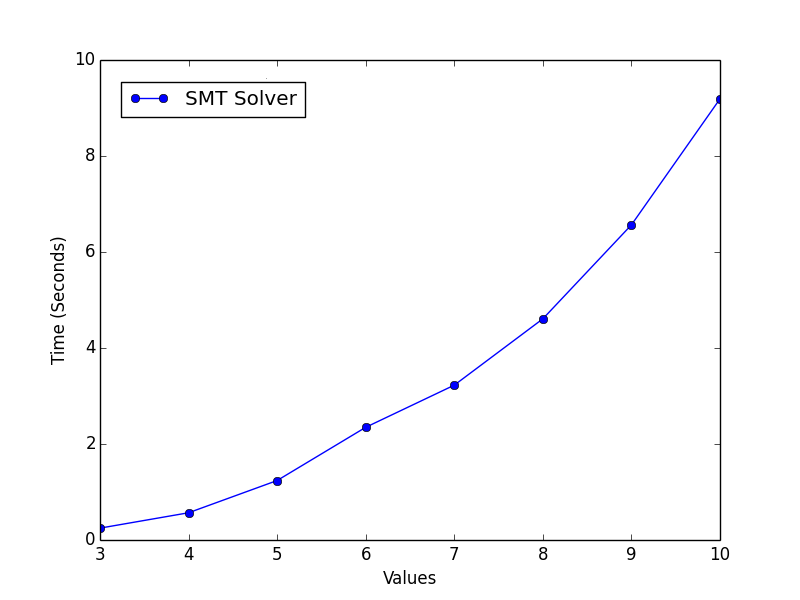
\includegraphics[width=.75\linewidth]{SMTOnlyVAL-v345678910p4n5.png}
\caption{4 Properties and 5 Sets Found Varying the Number of Values}
\label{fig:SMTVal}
\end{minipage}
\end{figure}



\subsection{Varying the Number of Properties}

Again, the SMT solver is able to finish larger instances of the problem faster than the dynamic algorithm past a certain threshold. See Figure~\ref{fig:DvSPROP}. Only once the number of properties increases past 5 is the SMT solver significantly faster than the dynamic algorithm. At this threshold, the dynamic algorithm takes much too long and it becomes only feasible to run the SMT solver by itself. 


The SMT solver is able to handle much larger number of properties than the dynamic algorithm without growing exponentially till a later degree. Once the number of properties is increased to 7, the SMT solver also begins to grow exponentially. See Figure~\ref{fig:SMTProp}.

\begin{figure}[htbb]
\begin{minipage}[b]{0.5\linewidth}
\centering
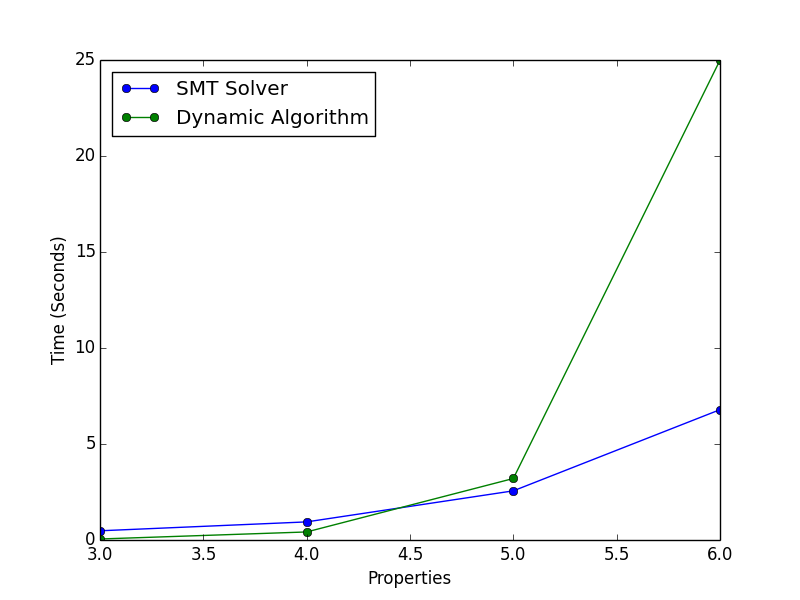
\includegraphics[width=.75\linewidth]{DvSPROP-v4p3456n10.png}
\caption{4 Values and 10 Sets Found Varying the Number of Properties}
\label{fig:DvSPROP}
\end{minipage}
\hspace{0.5cm}
\begin{minipage}[b]{0.5\linewidth}
\centering
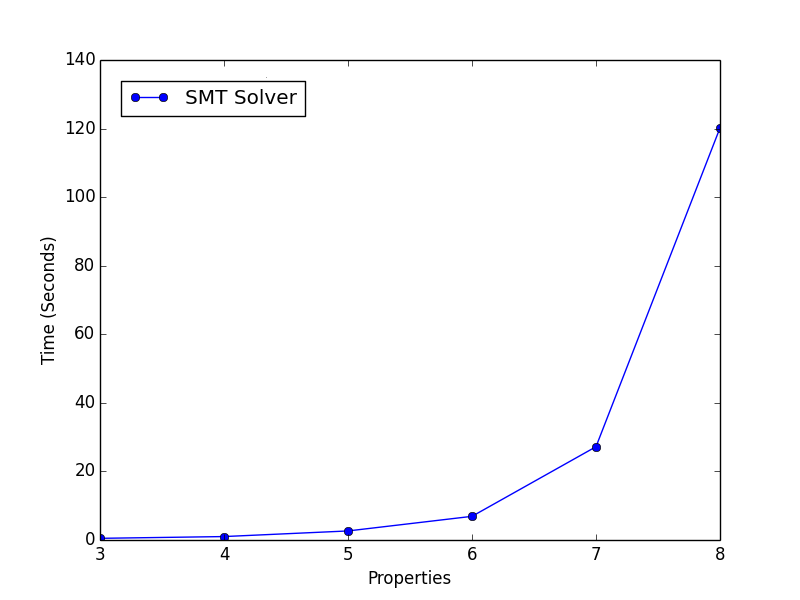
\includegraphics[width=.75\linewidth]{SMTOnlyPROP-v4p345678n10.png}
\caption{4 Values and 10 Sets Found Varying the Number of Properties}
\label{fig:SMTProp}
\end{minipage}
\end{figure}





\subsection{Varying the Number of Sets to be Found}

As the number of sets to be found increases, if the number of values and properties is high enough, the dynamic algorithm is much slower than  the SMT solver. See Figure~\ref{fig:DvSSETS}. Even though the dynamic algorithm creates a speed up by retaining all partial sets especially for multiple draws, the speed up does not always outweigh the cost of storing so many partial sets.

As the number of sets increases, the growth of both the SMT solver and dynamic algorithm are roughly identical. However, the SMT solver is marginally faster. The runtime continues to grow linearly in Figure~\ref{fig:SMTSet} as it finds more sets than in the previous figure with the same constant parameters.


\begin{figure}[htbb]
\begin{minipage}[b]{0.5\linewidth}
\centering
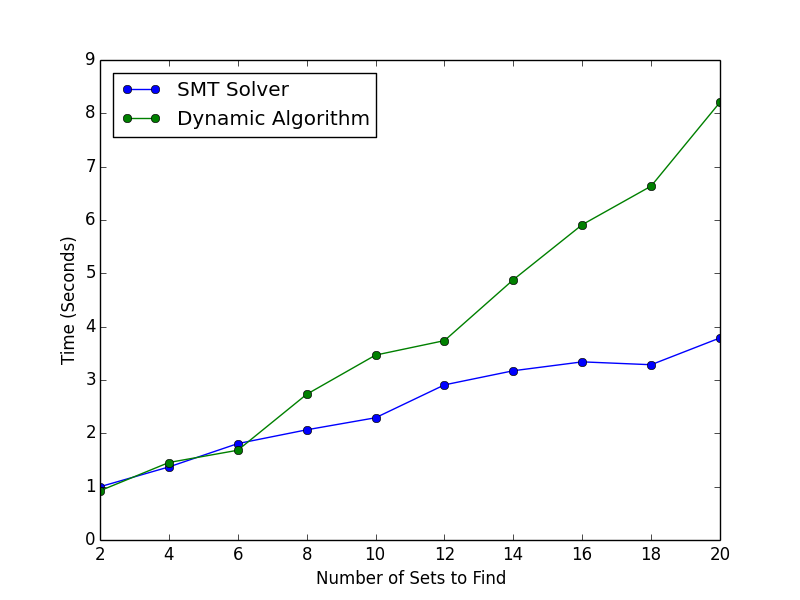
\includegraphics[width=.75\linewidth]{DvSSETS-v4p5n2468101214161820.png}
\caption{4 Values and 5 Properties Varying the Number of Sets to Find}
\label{fig:DvSSETS}
\end{minipage}
\hspace{0.5cm}
\begin{minipage}[b]{0.5\linewidth}
\centering
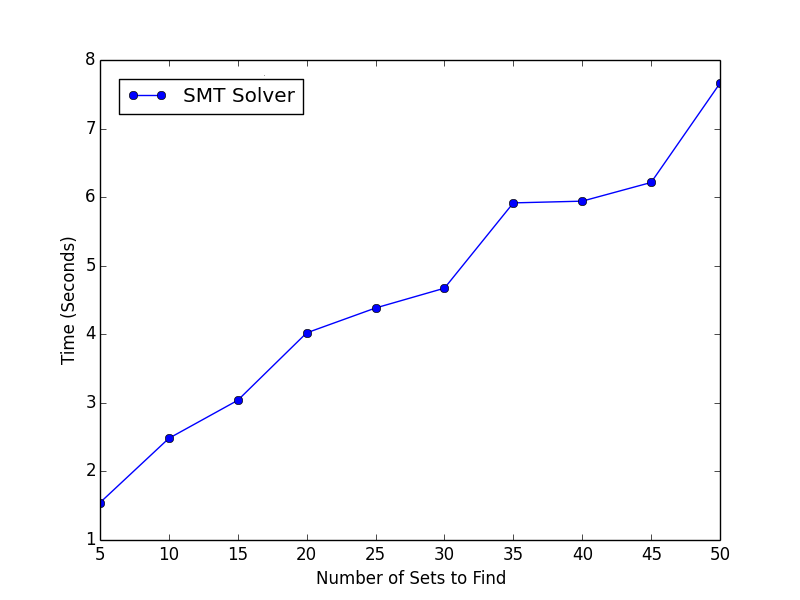
\includegraphics[width=.75\linewidth]{SMTOnlySETS-v4p5n5101520253035404550.png}
\caption{4 Values and 5 Properties Varying the Number of Sets to Find}
\label{fig:SMTSet}
\end{minipage}
\end{figure}

\section{Conclusion and Future Work}


This paper outlines the creation of three different solvers: brute force, dynamic algorithm, and SMT based, to solve the generalized Game of Set. Through timing tests, I found that as expected, the brute force implementation blows up exponentially as any of the parameters are increased. It does not lend itself to be an efficient solver for the more general case. The dynamic algorithm and SMT based solver both perform much better than the brute force and are superior in their own ways. The dynamic algorithm is faster on smaller cases than the SMT solver, but as the parameters increase, the memory usage of the dynamic algorithm become too unwieldy and causes it be much slower, exponentially increasing. Interestingly, only when the SMT solver is used on higher number of properties does its growth take on exponential growth. Otherwise, in the case of the values and sets to find, the SMT solver can continue its linear growth till much higher values. 

For future research into this problem, it would be interesting and potentially much faster if there is a way to combine the SMT solver and dynamic algorithm. This way, we could benefit from the dynamic algorithm's speed on smaller cases but also the SMT solver's efficiency for larger cases. If a solution combining the two can be found and implemented, this line of thinking could be very useful in creating efficient solutions for other problems that grow exponentially and need an efficient solver for a wide range of parameters. 


%One way to do this would be to run both algorithms in parallel and whichever one returns first will be a set. The only issue would be the bookkeeping would be much harder as we would constantly need to change the constraints for the SMT or the partial sets in the dynamic algorithm.
\section{Acknowledgments}

Thank you to Professor Kincaid for guidance and support through this project. 

\section{Ethics}

I pledge my honor that this project represents my own work in accordance with University regulations.

Steven Takeshita



\bstctlcite{bstctl:etal, bstctl:nodash, bstctl:simpurl}
\bibliographystyle{IEEEtranS}
\bibliography{references}

\section{Appendix}

All code is hosted on \url{https://github.com/steventakeshita/IW_Spring_2017}.

\end{document}